\documentclass[a4paper,12pt]{article}
\usepackage[a4paper]{geometry}
\usepackage{polski}
\usepackage[polish]{babel}
\usepackage[utf8]{inputenc}
\usepackage{indentfirst}
\usepackage{graphicx}
\usepackage{lastpage}
\usepackage{fancyhdr}
\usepackage{hyperref}
\usepackage{float}
%head & foot
\pagestyle{fancy}
\title{Specyfikacja funkcjonalna projektu \textit{Gra w Życie} w~języku C}
\author{Chabik Jan (291060), Łuczak Mateusz (291088)}
\date{8 marca 2018}
\setlength\parindent{24pt}
\setlength{\headheight}{16pt}
\lhead{}
\rhead{Specyfikacja funkcjonalna projektu \textit{Gra w Życie} w języku C}
\rfoot{str. \thepage/\pageref{LastPage}}
\cfoot{}

\begin{document}
\maketitle
\thispagestyle{empty}
\begin{center}
	
\includegraphics[scale=0.1]{logo_ee_big.png}
\end{center}
\newpage

\tableofcontents
\pagenumbering{arabic}
\newpage

\section{Opis ogólny}
\subsection{Nazwa programu}

Program nazwany został \texttt{Life}. Nazwa nawiązuje do rozwiązywanego problemu, którym jest stworzenie emulatora \textit{Gry w Życie} Johna Conwaya.

\subsection{Poruszany problem}
Poruszanym problemem będzie stworzenie emulatora \textit{Gry w Życie} Johna Conwaya w języku C.

\textit{Gra w życie} jest jednym z pierwszych i najbardziej znanych automatów komórkowych. Pozwala ona zrozumieć koncepty matematyczne takie jak układy sąsiadów i reguły zmian, a rozgrywa się na planszy, na której istnieje skończona ilość komórek. Każda z nich może się znajdować w stanie "żywym"\ lub "martwym". W~jednostce czasowej, każdej komórce przypisywany jest stan na podstawie stanów jej sąsiadów. Rozwiązaniem będzie $N$ wygenerowanych plików opisujących kolejne generacje automatu komórkowego dla zadanego przez użytkownika wejścia.

\subsection{Cel projektu}
Celem projektu jest zapoznanie się przez studentów z problemem \textit{Gry w Życie} Johna Conwaya oraz stworzenie implementacji w języku C. Zadanie przewidziane zostało dla grup dwuosobowych. Ze względu na to, ważna jest umiejętność pracy w zespole.

\section{Opis funkcjonalności}

\subsection{Korzystanie z programu}
Program po skompilowaniu powinien zostać uruchomiony w środowisku tekstowym wraz z koniecznymi argumentami opisującymi przykładowo plik wejściowy, plik docelowy, wybór sąsiedztwa czy ilość generacji automatu komórkowego.

\subsection{Uruchomienie programu}
Przy kompilacji programu za pomocą programu \texttt{Make} zostanie utworzony plik wynikowy \texttt{gameoflife}.

\texttt{./gameoflife <input\_file.txt> <katalog\_wyjsciowy> [-s 1/2] [-n \\ilosc\_generacji] [-g numer\_pierwszej] [-d] [-h --help]}
\begin{itemize}
	\item	\texttt{<input\_file.txt>} - Plik wejściowy w formacie .txt zawierający dane dotyczące mapy automatu komórkowego. Zawiera on wymiary macierzy oraz informacje o występowaniu żywych komórek.
    \item	\texttt{<katalog\_wyjsciowy>} - Katalog, w którym zostaną zapisane dane wynikowe programu w formacie \texttt{.txt} oraz \texttt{.png}.
    \item	\texttt{[-s sasiedztwo]} - Wybór pomiędzy wykorzystaniem sąsiedztwa Moore'a (1) i sąsiedztwa von Neumanna (2). W przypadku, jeżeli nie został użyty ten argument wywołania, zostanie użyte sąsiedztwo domyślne zapisane w kodzie źródłowym programu.
    \item	\texttt{[-n ilosc\_generacji]} - Ilość generacji do stworzenia. W przypadku, jeżeli nie został użyty ten argument wywołania, zostanie użyta domyślna wartość zapisana w kodzie źródłowym programu.
    \item	\texttt{[-g numer\_pierwszej]} - Numer pierwszej generacji (z pominięciem wprowadzanej przez dane wejściowe; ona zostanie uznana jako generacja 0). W~przypadku, jeżeli nie został użyty ten argument wywołania, zostanie użyta domyślna wartość zapisana w kodzie źródłowym programu.
    \item	\texttt{[-d]} - Ustawienie dialogu z użytkownikiem. Przy użyciu tego argumentu, po każdej stworzonej generacji, program będzie pytał użytkownika, czy ma zostać zapisana do pliku \texttt{.txt} oraz \texttt{.png}. Domyślnie, bez użycia argumentu, opcja jest wyłączona.
    \item 	\texttt{[-h]} lub \texttt{[--help]} - Wyświetlenie składni programu. Nie może być uruchomiony z innymi argumentami.
\end{itemize}

\subsection{Możliwości programu}
\begin{itemize}
\item Emulacja \textit{Gry w Życie} Johna Conwaya;
\item Odczyt danych z pliku tekstowego zawierającego informacje dotyczące mapy automatu komórkowego;
\item Generowanie wybranej przez użytkownika ilości generacji automatu komórkowego;
\item Symulacja automatu dla wybranego przez użytkownika sąsiedztwa (wybór spośród sąsiedztwa Moore'a i von Neumanna);
\item Zapis danych wyjściowych do pliku tekstowego oraz pliku \texttt{.png};
\item Wyświetlanie planszy do terminala oraz  możliwość zapisu do \texttt{.png} na życzenie (gdy wybierzemy opcję dialogu z użytkownikiem).
\end{itemize}

\section{Format danych i struktura plików}
\subsection{Słownik pojęć}
\begin{itemize}
\item \textbf{Plasza} - jest to prostokąt podzielony na pola (komórki), z których każda ma przypisaną wartość - 0 albo 1. Gdy komórka znajduje się stanie '0' mówimy, że jest martwa, w przeciwnym wypadku jest żywa;
\item \textbf{Sąsiedztwo Moore'a} - typ sąsiedztwa polegający na tym, iż rozpatrywane są wszystkie 8 komórek sąsiadujących z daną komórką (komórka na północ, południe, wschód, zachód, północny-wschód, północny-zachód, południowy-zachód, południowy-wschód);
\begin{figure}[H]
	\centering
    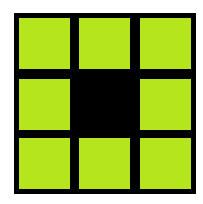
\includegraphics[scale=1]{moore.png}
    \caption{Sąsiedztwo Moore'a. Po środku znajduje się komórka (czarna), dla której rozpatrujemy sąsiadów. Komórki zielone opisują, które z nich są sąsiadami w opisywanym sąsiedztwie.}
\end{figure}
\item \textbf{Sąsiedztwo Von Neumanna} - typ sąsiedztwa polegający na tym, iż rozpatrywane są 4 komórki sąsiadujące (komórka na północ, południe, wschód i zachód);
\begin{figure}[H]
	\centering
    
\includegraphics[scale=1]{von_neumann.png}
    \caption{Sąsiedztwo von Neumanna. Po środku znajduje się komórka (czarna), dla której rozpatrujemy sąsiadów. Komórki zielone opisują, które z nich są sąsiadami w opisywanym sąsiedztwie.}
\end{figure}
\end{itemize}
\subsection{Struktura katalogów}
\noindent\texttt{.\\
|\\
+- /C/docs} - Katalog z dokumentami projektowymi\\\texttt{
|\\
+- /C/bin} - Katalog z danymi wyjściowymi kompilacji programu\\\texttt{
|\\
+- /C/src} - Katalog z kodami źródłowymi programu\\\texttt{
|\\
+- /C/tests} - Katalog z testami dla programu\\\texttt{
|\\
+- /C/mod\_tests} - Katalog z testami modułów i funkcji programu


\subsection{Przechowywanie danych w programie}
\begin{itemize}
\item Dane na temat planszy przechowujemy w tablicy typu char, celem oszczędności pamięci. 
\item Program przechowuje wskaźnik do pliku, z którego ``czyta"\ dane oraz wskaźnik do katalogu, do którego dodaje pliki \texttt{.png} i \texttt{.txt};
\end{itemize}

\subsection{Dane wejściowe}
Jako dane wejściowe służy plik w formacie \texttt{.txt}, w którym zapisana jest plansza.

Plik rozpoczyna się wymiarami planszy zapisanej za pomocą liczb naturalnych większych od 0. Następnie podawane są cyfry '0' i '1' oznaczające stan komórki (martwa lub żywa). Ilość cyfr powinna odpowiadać wielkości planszy. Przykładowo, jeżeli wymiary macierzy to \texttt{3x4}, to powinno być podanych 12 cyfr oznaczających stan komórek.


\subsection{Dane wyjściowe}
\begin{itemize}
\item Pliki \texttt{.png}, w których znajduje się graficzna interpretacja każdej kolejnej generacji;
\item Pliki w formacie \texttt{.txt}, w których zapisane są kolejne generacje;
\item W przypadku uruchomienia opcji dialogu z użytkownikiem, dane wyjściowe będą wypisywane również w oknie terminala.
\end{itemize}


\section{Scenariusz działania programu}
\subsection{Scenariusz ogólny}
\begin{enumerate}
\item Uruchomienie programu z terminala z argumentami określającymi dalsze jego działanie;
\item Sprawdzenie przez program argumentów oraz poprawności danych wejściowych;
\item Zapisanie danych z argumentów do pamięci programu;
\item Stworzenie mapy automatu komórkowego;
\item Tworzenie kolejnych generacji automatu;
\item W przypadku wybrania możliwości dialogu z użytkownikiem:
	\begin{itemize}
    \item Wyświetlenie stworzonej generacji na ekranie powłoki tekstowej;
	\item Pytanie o zezwolenie na zapis danych wyjściowych do \texttt{.txt} i \texttt{.png};
    \item Ewentualny zapis lub pomięcie zapisu danej generacji.
    \end{itemize}
\item W przypadku uruchomienia programu bez opcji dialogu z użytkownikiem, zapis danych zgodnie z podanymi argumentami lub wartościami domyślnymi;
\item Po każdym zapisie, utworzenie nowej mapy na podstawie zmian automatu komórkowego i powtórzenie kroków 6 lub 7 (zależnie od sposobu uruchomienia programu);
\item Zakończenie pracy programu z komunikatem o ukończeniu pracy.
\end{enumerate}

\subsection{Scenariusz szczegółowy}
\begin{enumerate}
\item Uruchomienie programu z terminala z argumentami określającymi dalsze jego działanie:
	\begin{itemize}
	\item W przypadku podania błędnych danych wejściowych (błędne argumenty) program zostaje przerwany oraz zostaje wyświetlona poprawna składnia programu, oraz pomoc;
    \item W przypadku podania nieistniejącego pliku wejściowego, lub braku uzyskania do niego dostępu, program zakończy się z komunikatem o błędzie.
    \end{itemize}
\item Sprawdzenie przez program argumentów oraz poprawności danych wejściowych:
	\begin{itemize}
    \item Sprawdzenie danych wejściowych pod kątem błędnych informacji na temat mapy automatu komórkowego. W przypadku znalezienia nieprawidłowych znaków w macierzy (znaki niebędące opisem komórek, czyli inne niż '0' i '1') program zgłosi problem użytkownikowi, a tym samym jego działanie się zakończy.
    \end{itemize}
\item Zapisanie danych z argumentów do pamięci programu:
	\begin{itemize}
    \item Zapisanie danych z argumentów do zmiennych i tablic w programie.
    \end{itemize}
\item Stworzenie mapy automatu komórkowego:
	\begin{itemize}
    \item Stworzenie planszy na podstawie podanych danych wejściowych.
    \end{itemize}
\item Tworzenie kolejnych generacji automatu:
	\begin{itemize}
    \item Na podstawie wybranego sąsiedztwa, tworzenie kolejnych generacji po przejściach komórek zgodnie z wybranym typem sąsiedztwa.
    \end{itemize}
\item W przypadku wybrania możliwości dialogu z użytkownikiem:
	\begin{itemize}
    \item Wyświetlenie stworzonej generacji na ekranie powłoki tekstowej;
	\item Pytanie o zezwolenie na zapis danych wyjściowych do \texttt{.txt} i \texttt{.png};
    \item Ewentualny zapis lub pomięcie zapisu danej generacji.
    \end{itemize}
\item W przypadku uruchomienia programu bez opcji dialogu z użytkownikiem, zapis danych zgodnie z podanymi argumentami lub wartościami domyślnymi:
	\begin{itemize}
    \item Na podstawie danych o ilości generacji i numerze pierwszej stworzonej generacji następuje zapis danych wynikowych do wybranego katalogu w formatach \texttt{.txt} i \texttt{.png}.
    \end{itemize}
\item Po każdym zapisie, utworzenie nowej mapy na podstawie zmian automatu komórkowego i powtórzenie kroków 6 lub 7 (zależnie od sposobu uruchomienia programu);
\item Zakończenie pracy programu z komunikatem o ukończeniu pracy.
\end{enumerate}

\section{Testowanie}
Testować będziemy każdą funkcję z osobna, potem każdy z modułów programu, a na końcu cały program. Testy będą “ręczne”, rezultaty będziemy sprawdzać z pomocą debuggera (gdb). Poprawność generacji planszy będziemy sprawdzać za pomocą strony \url{https://www.mimuw.edu.pl/~ajank/zycie/}, na której można śledzić działanie automatu komórkowego.

\end{document}
